\providecommand{\main}{../../..}
\documentclass[\main/dresen_thesis.tex]{subfiles}
\renewcommand{\thisPath}{\main/chapters/appendix/characterizationAcCoFeC2}
\begin{document}

\chapter{Characterization of Ac-CoFe-C-2}\label{app:characterizationAcCoFeC2}
  In \refsec{sec:monolayers:nanoparticle:structuralCharacterization}, nanocubes from acetylacetonates are extensively discussed and characterized by TEM, SAXS, SANS(POL), XRD and VSM.
  Due to the small yield of nanocubes it was necessary during this work to prepare a second batch, which is used in \refch{ch:monolayers} to discuss the lateral nuclear and magnetic structure of monolayers by grazing-incidence small-angle scattering, where the preparation has been to most part parallel to Ac-CoFe-C.
  To obtain insight into the single-particle properties, all characterization experiments have also been performed for Ac-CoFe-C2 and are presented here in the following.

  \begin{figure}
    \centering
    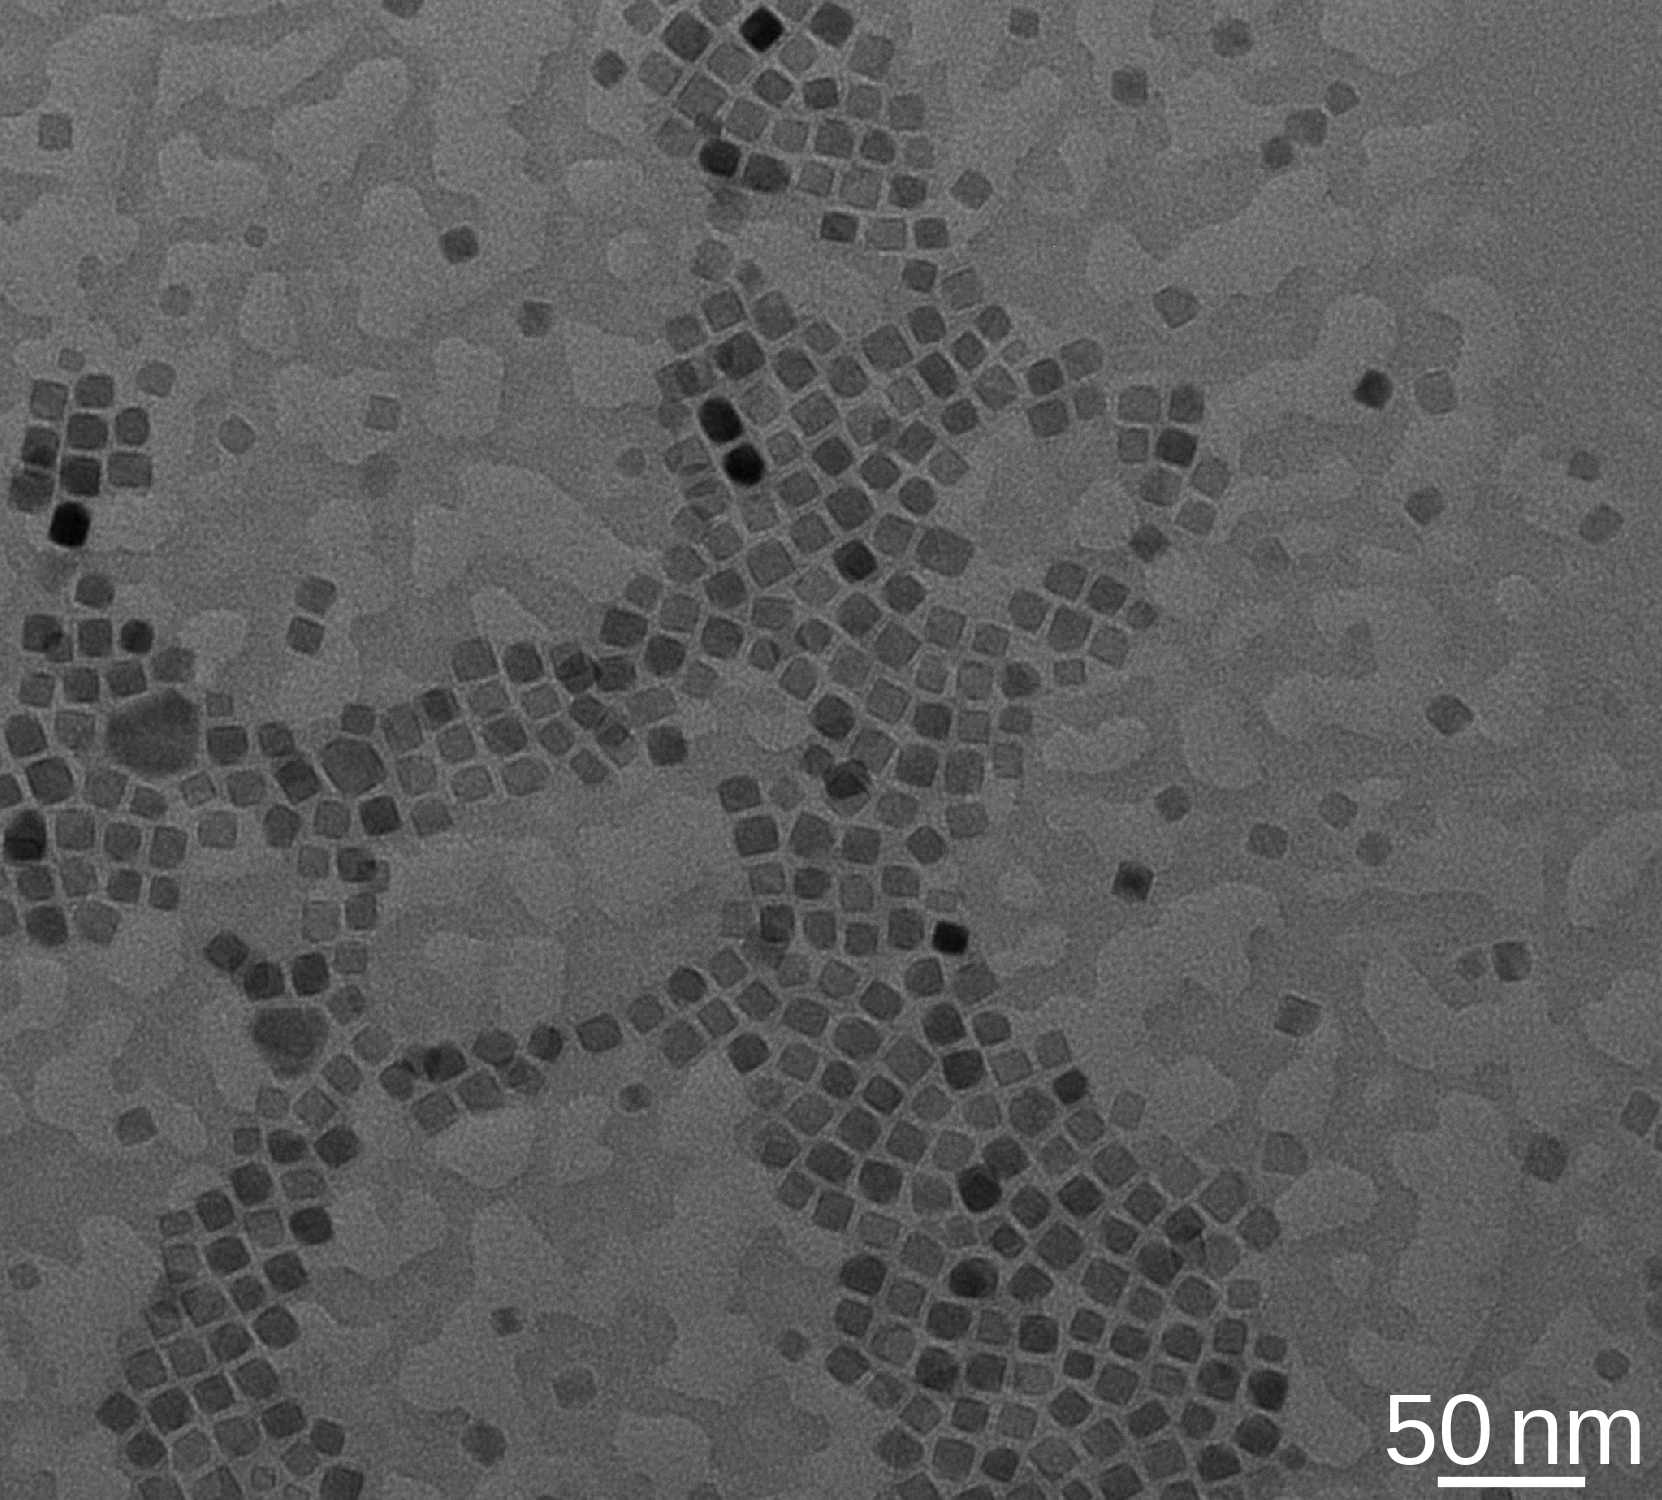
\includegraphics{appendix_characAcCoFeC2_TEM_Ac_CoFe_C_2}
    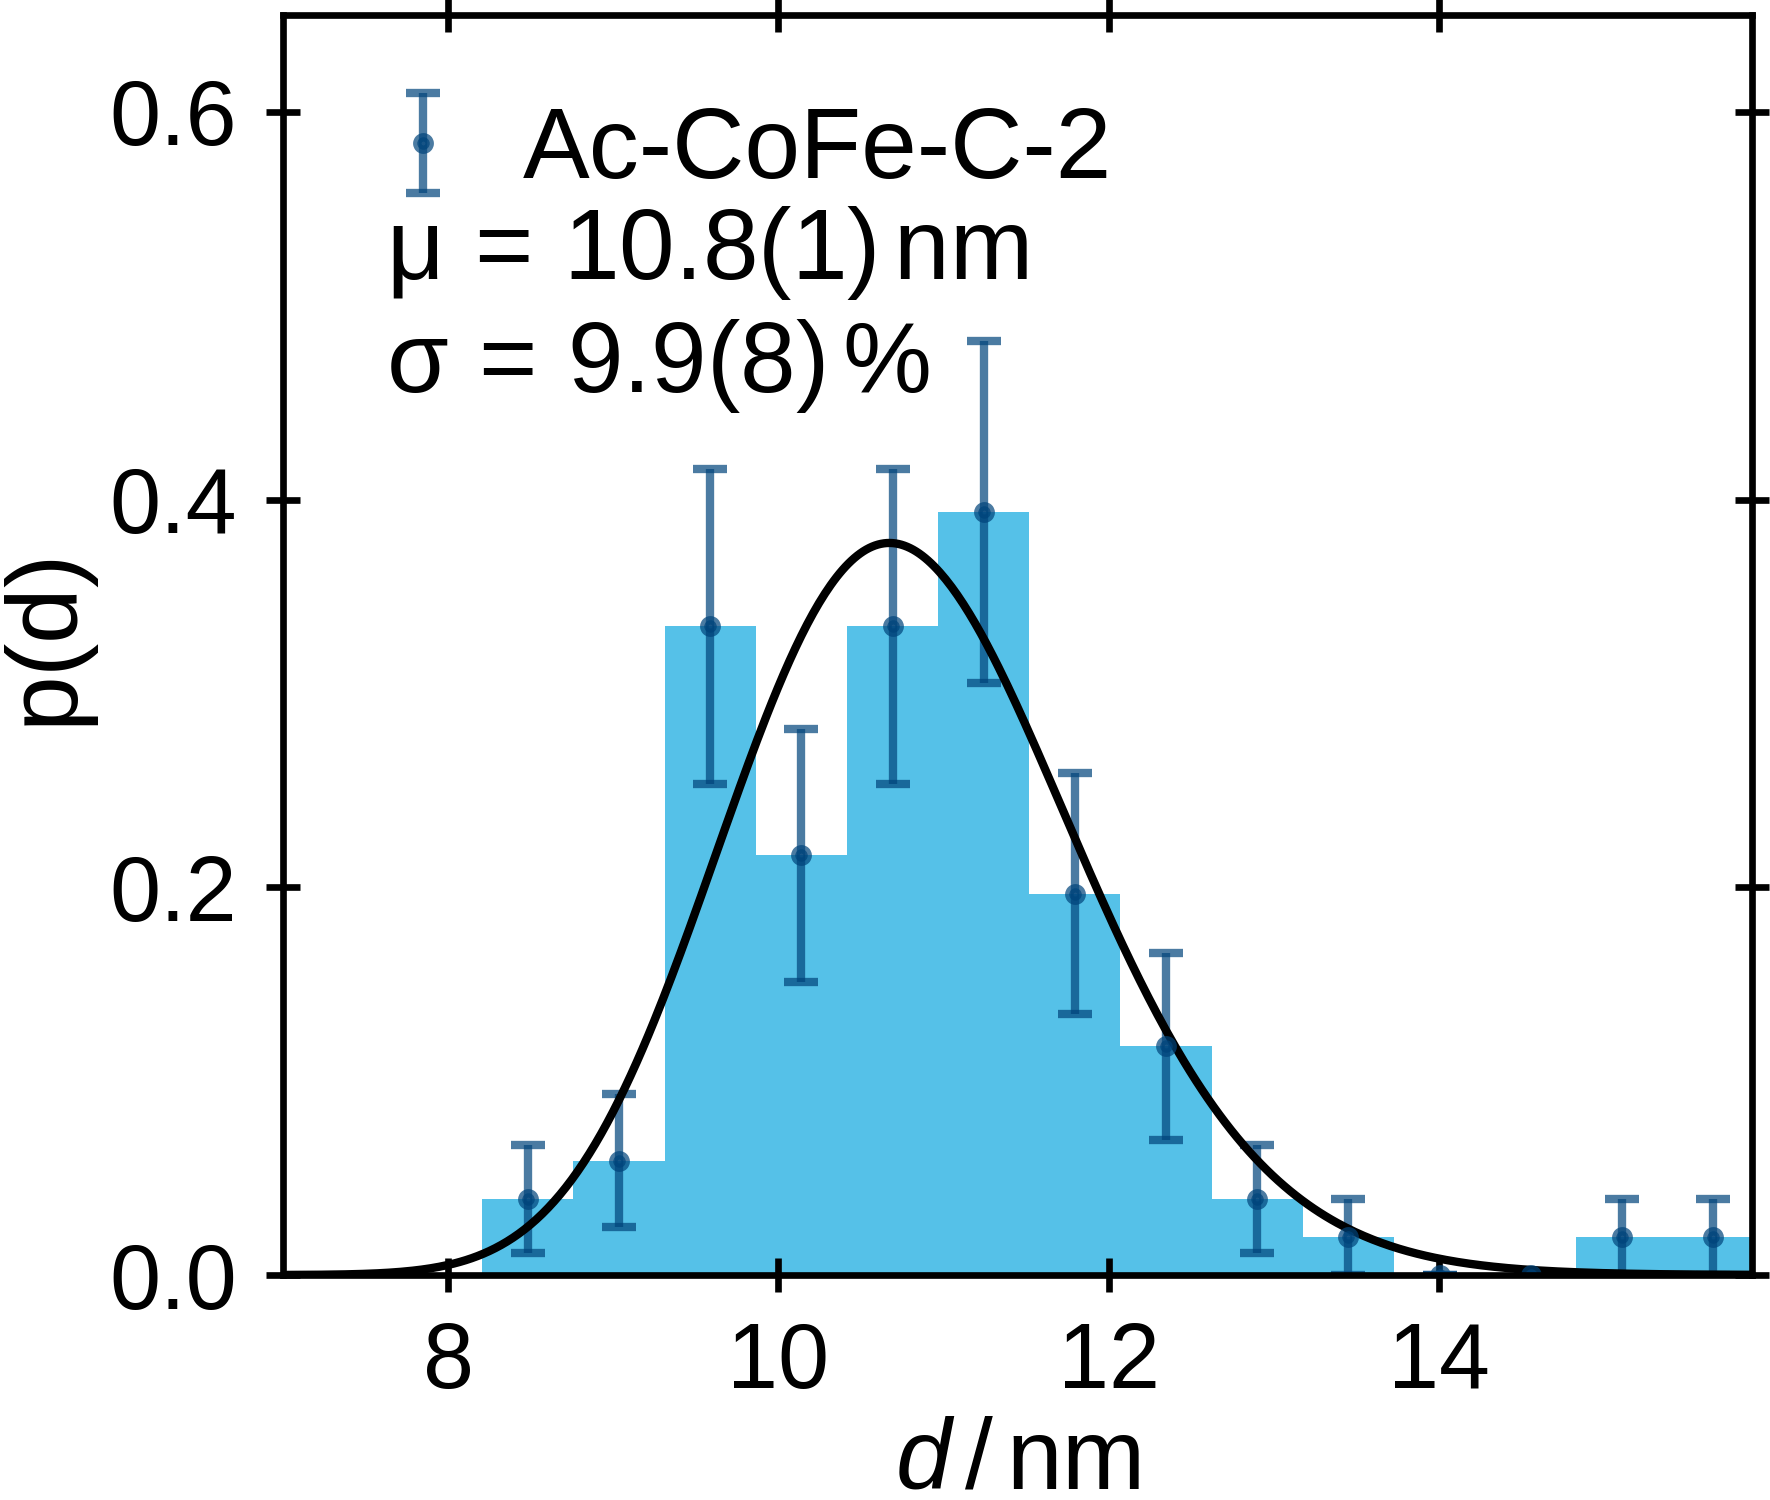
\includegraphics{appendix_characAcCoFeC2_TEM_Ac_CoFe_C_2_sizeDist}
    \caption{\label{app:characterizationAcCoFeC2:TEM}TEM micrograph and extracted size distribution from counting the frequencies of the edge lengths.}
  \end{figure}


  \begin{figure}
    \centering
    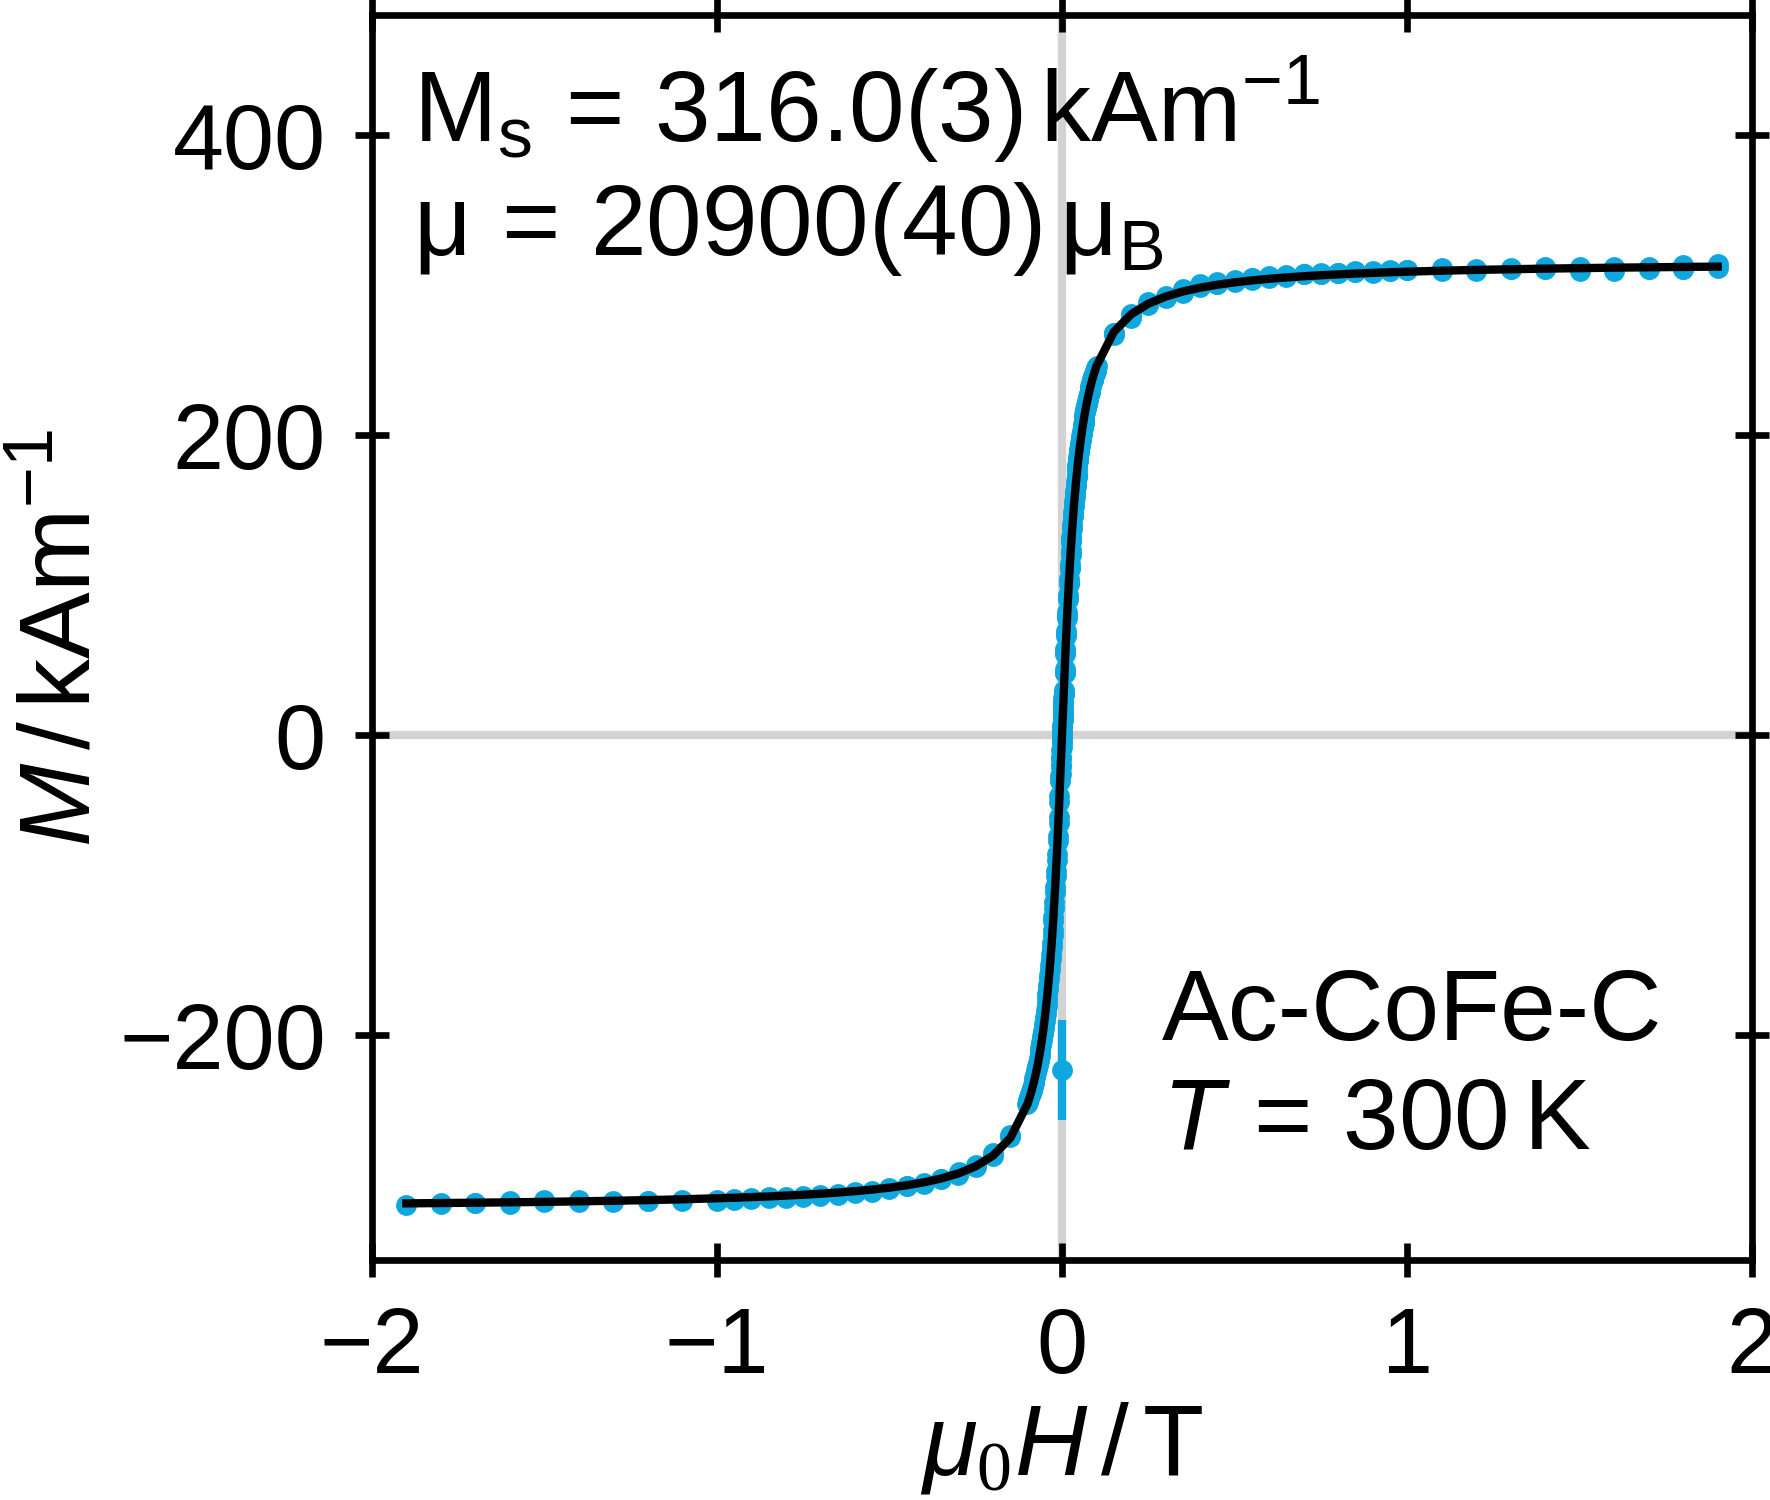
\includegraphics{appendix_characAcCoFeC2_VSM_Ac_CoFe_C_2}
    \caption{\label{app:characterizationAcCoFeC2:VSM}VSM.}
  \end{figure}
  \begin{figure}
    \centering
    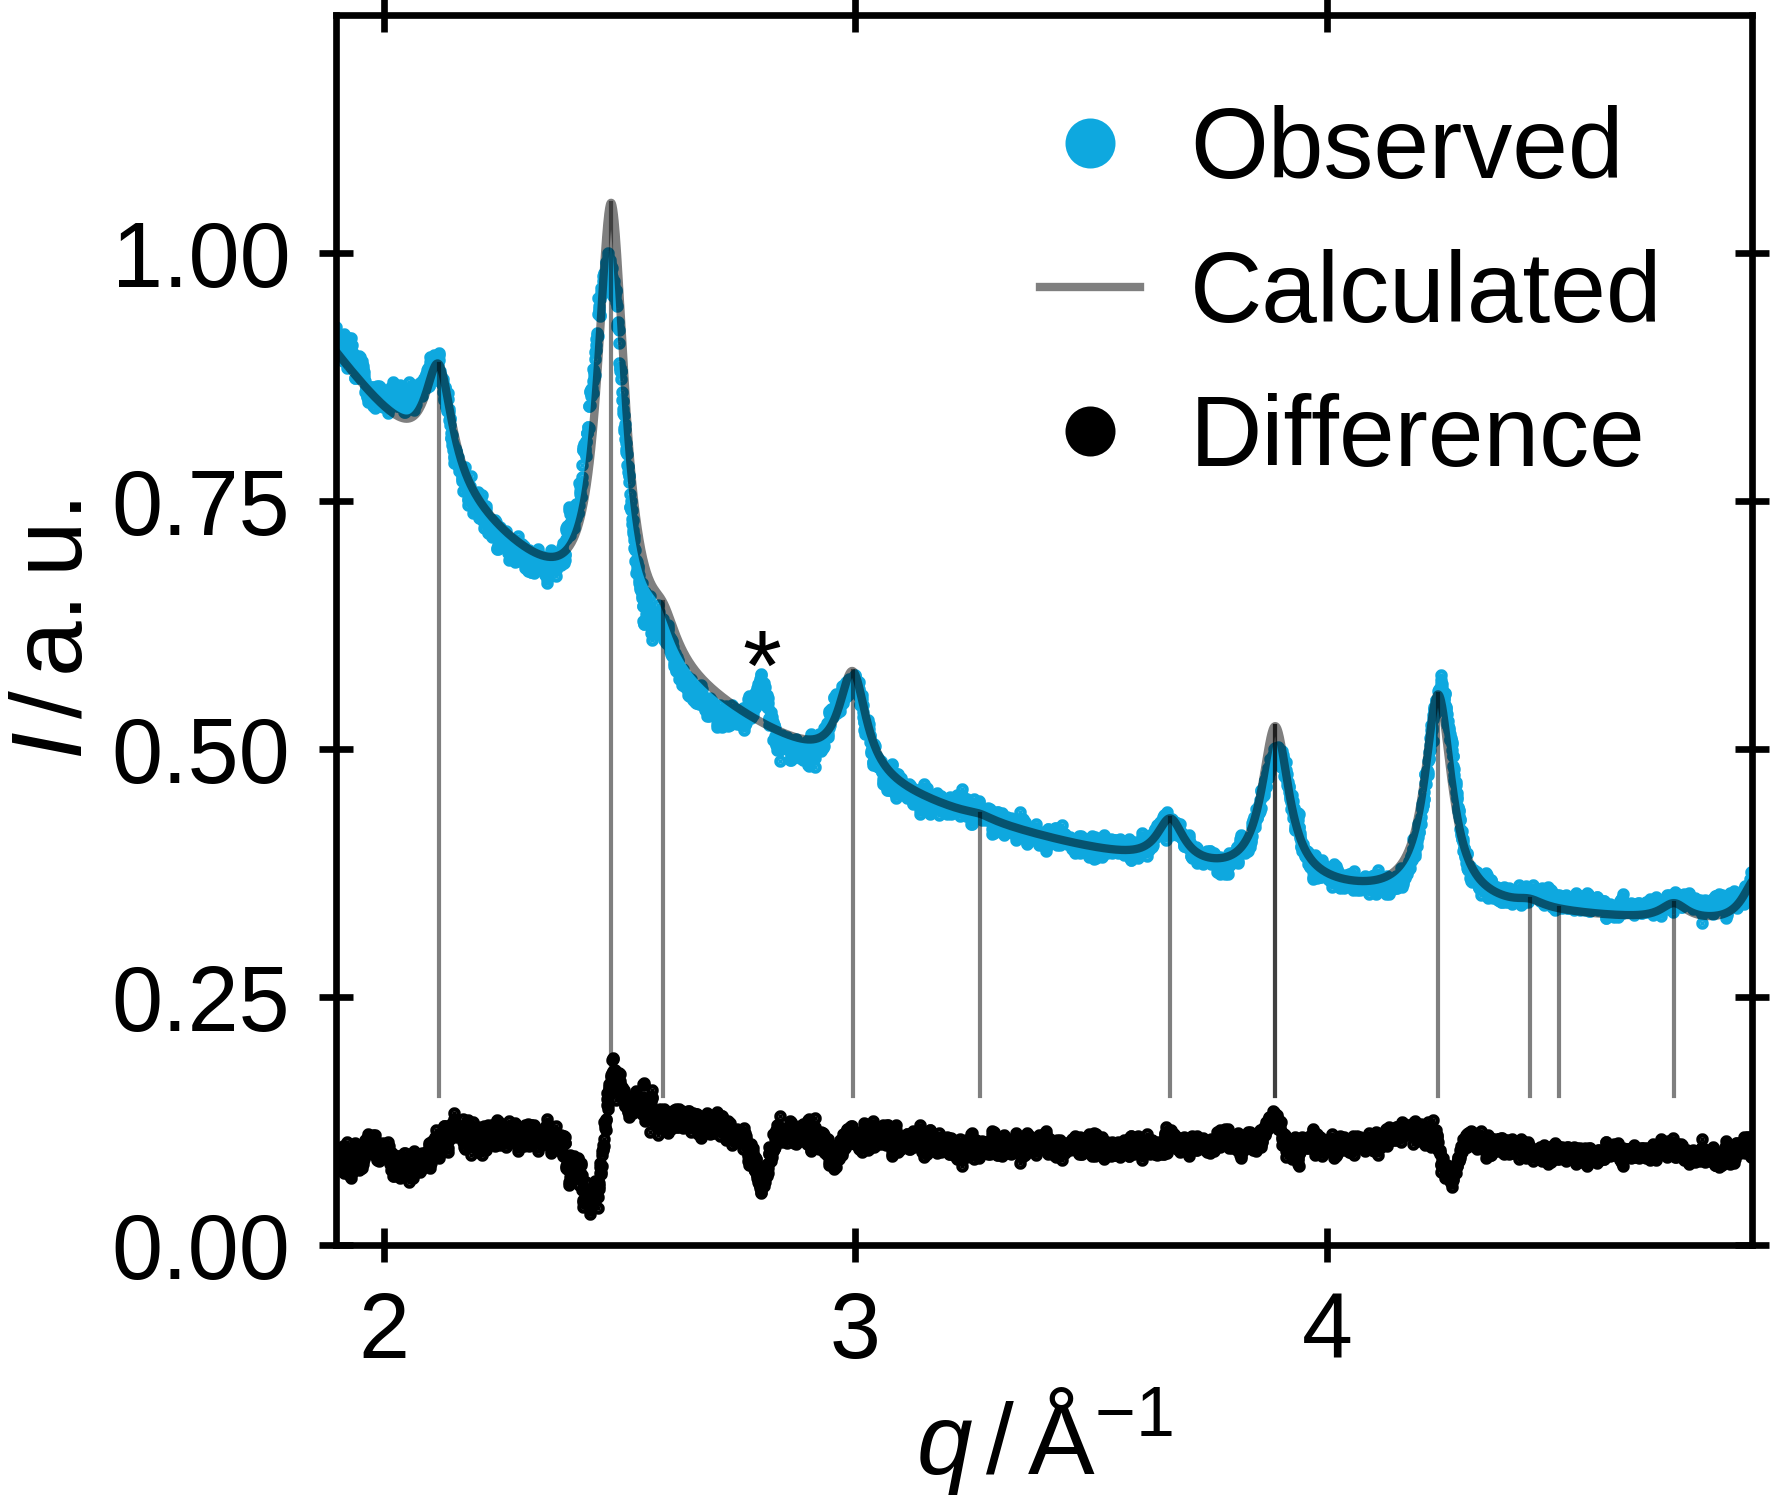
\includegraphics{appendix_characAcCoFeC2_XRD_Ac_CoFe_C_2}
    \caption{\label{app:characterizationAcCoFeC2:XRD}XRD.}
  \end{figure}
  
  
\end{document}